In order to be able to perform a similarity assessment between queries, activities, and sessions, we need to be able to extract features out of SQL queries.
%, compare them and compute pairwise similarity between them.
Extracting features from a SQL query can be done in many ways. Let's consider the following queries:

\begin{verbatim}
Q1: SELECT username FROM user WHERE rank = "admin"
 
Q2: SELECT rank, count(*) FROM user
    WHERE rank <> "admin" GROUP BY rank
\end{verbatim}

These two queries share many attributes, and seem to be working on similar concepts although not performing semantically very similar tasks. Usually, what we consider important in a query can roughly be listed as \textit{selection}, \textit{joins}, \textit{group-by}, \textit{projection}, and \textit{order-by}.

Makiyama \textit{et al.}~\cite{makiyama2015text} put forward the most similar work we are working on. They perform query log analysis with a motivation of analyzing the workload on the system, and they provide a set of experiments on Sloan Digital Sky Survey (SDSS) dataset. They extract the terms in \textit{selection}, \textit{joins}, \textit{projection}, \textit{from}, \textit{group-by}, and \textit{order-by} items separately, and create the query vector out of their appearance frequency for each query in the dataset. They compute the pairwise similarity of queries with cosine similarity.

\begin{figure}[h!]
    \centering
    \includegraphics[width=0.5\textwidth]{graphics/clustering}
    \caption{The workflow for clustering process}
    \label{fig:clusteringWorkflow}
\end{figure}

%To clarify the ambiguity between distance and similarity terms, we define distance as follows:

%$$distance = 1 - similarity$$

%where the similarity is the score we get from the methods explained above. 

The \emph{profiles} to compare activities and sessions can be performed in three ways: (1) Feature based sets which can be compared with Jaccard Index, (2) KL-Divergence entropy using feature appearance frequencies, and (3) Jaccard Index using the clustering appointments of queries.

\tinysection{Feature sets based Jaccard Index} The Jaccard similarity coefficient is a statistic used for comparing the similarity and diversity of sample sets. The Jaccard coefficient measures similarity between finite sample sets, and is defined as the size of the intersection divided by the size of the union of the sample sets. For two user sessions $S_i$ and $S_j$, we compare the feature sets of these sessions that are extracted from the constituent queries.

$$J(S_i,S_j) = \frac{\left[S_i\cap S_j\right]}{\left[S_i\cup S_j\right]}$$

If $S_i$ and $S_j$ are both empty, we define $J(S_i,S_j) = 1$. Also, this guarantees that $0\leq J(S_i,S_j) \leq 1$.


\begin{figure}[h!]
    \centering
    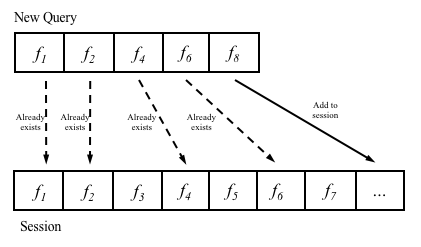
\includegraphics[width=0.5\textwidth]{graphics/featurebased.png}
    \caption{Creating a feature set based session profile}
    \label{fig:featureBasedSessionProfile}
\end{figure}

%We calculate $J(S_i,S_j)$ for all pairs of user sessions.

%Now, we start to look for "interesting" user sessions. One notion of of user sessions being interesting can be that their contents occur in the query log more frequently. A high Jaccard similarity score for a pair of user sessions can be interpreted as them being similar to each other, thereby leading the contents to occur more frequently. For a particular user session $w_i$, we would be now looking out for the top K user sessions which are most similar with $w_i$. Calculating the average similarity of $w_i$ with the most similar K sessions $[w_1,w_2..., w_k]$ yields a notion of the importance of $w_i$ in representing the characteristics of the workload represented in the query log. We denote this average similarity for $w_i$ with top K windows as $J_{w_i{avg}}$.

%$$J_{wi_{avg}}= \frac{\sum_{j=1}^{k} J(w_i,w_j)}{k}$$

%When we calculate $J_{w_i{avg}}$ for all $w_1,w_2...,w_m$, we obtain a vector of average similarity scores for the entire query log for a user.


\tinysection{KL-Divergence entropy} Each query $Q^{t_i}_u$ is processed with the methodology given above, and denoted as:

\begin{equation}
Q^{t}_u = ( f^{t}_1(c_0), f_2^{t}(c_1), ... , f_m^{t}(c_n) )
\end{equation}

where $t$ is the timestamp that the query $Q$ was issued, $u$ represents the username of the query owner, $f_i$ is the feature extracted, and $c_j$ denotes how many times the feature $f_i$ was observed in the query.

%Sessions over time may show various characteristics over time, and it is important to identify sessions that deviate from the other sessions to be able to generate new workloads.
%The generated workloads should reflect the normal behavior of users, but they should still include realistic deviations in order to create a pragmatic workload that emulate a user.

A session $S$ is represented by a user $u \in U$, where $U$ is the set of all users, for the time period $T$ that starts from $t_0$ and goes on for $\Delta t$, and the set of queries $Q$ performed by $u$ within $T$. Formally,

\begin{equation}
S^T_u = ( Q^{t_0}_u, Q^{t_1}_u, ... , Q^{t_n}_u )
\end{equation}

where $Q^{t_i}_u$ represents a query $Q_{t_i}$ issued at time $t_i$ by user $u$.

The \textit{session profiles} are created with the accumulation of these features from the beginning to the end of the session.
Using the appearance frequency of these features, we calculate the appearance probability of each harvested feature.
This multinomial probability distribution of the features for each session constitutes the \textit{session distribution}.
A session distribution $\phi$ is formally denoted as:

\begin{equation}
\phi^T_u = ( P(f_0)^{T}_u, P(f_1)^{T}_u, ... , P(f_n)^{T}_u )
\end{equation}

where $P(f_i)^{T}_u$ represents the probability of encountering feature $f_i$ within the timeframe $T$ among all the operations performed by user $u$.



We compute the difference between distributions with KL- Divergence~\cite{kullback1951information}.
%~\cite{fuglede2004jensen}.
Comparison of a session with the other sessions using KL-Divergence gives the difference denoted as follows:

%\begin{equation}
%d^{T_1}_u (\phi^{T_1}_u || \phi^{T_2}_u) = \frac{1}{2} KL(\phi^{T_1}_u || \phi^{T_2}_u) + KL(\phi^{T_2}_u || \phi^{T_1}_u)
%\end{equation}

%where 

\begin{equation}
KL(\phi^{T_1}_u || \phi^{T_2}_u) = \sum_i \phi^{T_1}_u(i)  log_2 \frac{\phi^{T_1}_u(i)}{\phi^{T_2}_u(i)}
\end{equation}

\textbf{KL-Divergence} is used for comparing two probability distributions, $P$ and $Q$; and it ranges between 0 and $\infty$. $D_{JS}(P||Q)$ essentially represents the symmetric information loss when $P$ distribution is used to approximate $Q$.

Note that when $P(i) \neq 0$ and $Q(i) = 0$,  $D_{JS}(P||Q)=\infty$. For example, suppose, we have two distributions $P$ and $Q$ as follows: $P = \{ f_0: 3/10, f_1: 4/10, f_2: 2/10, f_3: 1/10 \}$ and $Q = \{ f_0: 3/10, f_1: 3/10, f_2: 3/10, f_4: 1/10 \}$. In this case, since $f_3$ is not a part of $Q$, the result would be $\infty$, which means these two distributions are completely different. 

To get past this problem, we can apply \textit{smoothing} (i.e., Laplace/additive smoothing), which is essentially adding a small constant $epsilon$ to the distribution, to handle zero values, without significantly impacting the distribution. After we apply smoothing, $D_{KL}(P||Q)$ becomes $1.38$.

\begin{figure}[h!]
    \centering
    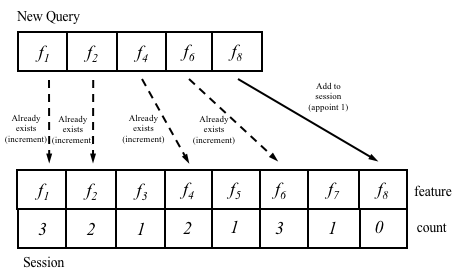
\includegraphics[width=0.5\textwidth]{graphics/entropy.png}
    \caption{Creating an probability distribution based session profile}
    \label{fig:entropySessionProfile}
\end{figure}

\tinysection{Jaccard Index using the clustering of queries} In this strategy, the profiler takes the preprocessed clustering appointments of queries as input instead of the features.

Clustering the queries in the workload narrows down the space of possible patterns that could be detected. This facilitates easier and more accurate understanding of the workload~\cite{pavlo2017self}. The main goal of this step is to group queries into classes that exhibit similar interests over database attributes. We consider two queries to exhibit similar interests over database attributes if they are similar in semantic structure. In the clustering process, we first filter the queries belonging to the app of our interest without distinguishing which user the activity belongs to. Then, we create clusters using all the queries belonging to that specific app. The workflow for the PocketData dataset is illustrated in Figure~\ref{fig:clusteringWorkflow}.

We use hierarchical clustering
%in our experiments,
which takes the distance matrix as input, and outputs a dendrogram -- a tree structure which shows how each query can be grouped together.
Furthermore, a dendrogram is a convenient way to visualize the relationship between queries and how each query is grouped in the clustering process.

To clarify the ambiguity between distance and similarity terms, we define distance as follows:

$$distance = 1 - similarity$$

where the similarity is the score we get from the methods explained above. 

\begin{figure}[h!]
    \centering
    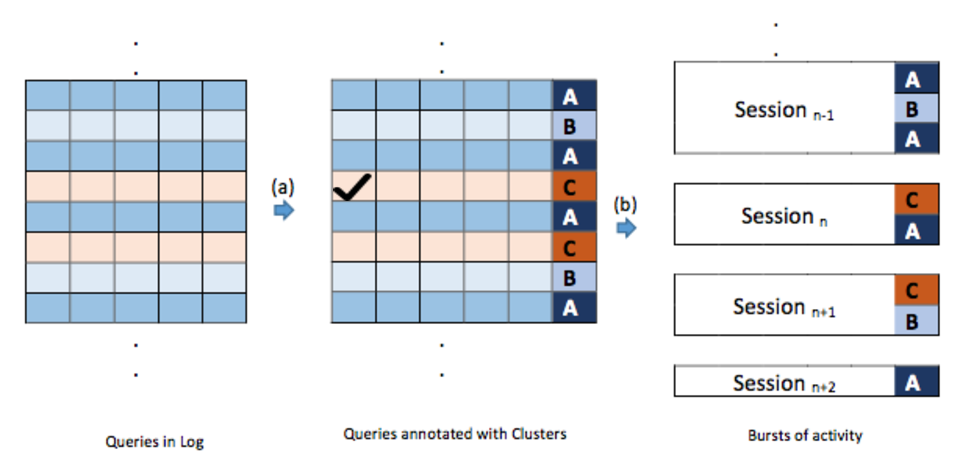
\includegraphics[width=0.5\textwidth]{graphics/systemoutline}
    \caption{Session representations with query clustering}
    \label{fig:clusterSession}
\end{figure}

In this form of session profiling, we embed query cluster appointments for all the queries within the session to the \emph{session profile}, which would be used to define the session for the rest of the process. An illustration of how the sessions are represented is given in Figure~\ref{fig:clusterSession}.

\todo{Show how to calculate the session similarity.}

\todo{Add a representative figure.}


